%! program = pdflatex

\documentclass[12pt,a4paper]{article} 
\usepackage{arc-dp}
\usepackage{amsfonts}
\usepackage{amsmath}
\usepackage{graphicx}
\usepackage{times}
\usepackage{setspace}
\usepackage{fancyhdr}
\usepackage{color}
\usepackage[normalem]{ulem}
\usepackage{subfig}
\usepackage{float}
\usepackage{caption}
\usepackage{array}
\usepackage{pgfgantt}
\usepackage{url}
\usepackage{enumitem}
\usepackage{subfig}
\usepackage{pgfgantt}
\usepackage{wrapfig}
\usepackage{enumitem}

\usepackage{booktabs} % for spacing tables
\usepackage{tabularx} % auto table sizing
\usepackage{multirow} % table multirow

%\usepackage{epsf}
%\usepackage{fancyheadings}
%\usepackage{subfigure}
%\usepackage{pst-gantt}
%\usepackage{tweaklist}

\newcolumntype{L}[1]{>{\raggedright\let\newline\\\arraybackslash\hspace{0pt}}m{#1}}
\newcolumntype{C}[1]{>{\centering\let\newline\\\arraybackslash\hspace{0pt}}m{#1}}
\newcolumntype{R}[1]{>{\raggedleft\let\newline\\\arraybackslash\hspace{0pt}}m{#1}}

\let\OLDthebibliography\thebibliography
\renewcommand\thebibliography[1]{
  \OLDthebibliography{#1}
  \setlength{\parskip}{1pt}
  \setlength{\itemsep}{1pt plus 0.3ex}
}


%\renewcommand{\enumhook}{\setlength{\topsep}{0pt}%
 % \setlength{\itemsep}{-2mm}}
%\renewcommand{\itemhook}{\setlength{\topsep}{0pt}%
%  \setlength{\itemsep}{-2mm}}
  %%%%%UNCOMMENT THE NEXT COMMAND IF NEEDED
%\renewcommand{\descripthook}{\setlength{\topsep}{0pt}%
%  \setlength{\itemsep}{-2mm}}

%\pagestyle{fancy}

%\input{psfig.sty}
\newcommand{\todo}[1]{\textcolor{red}{#1}}
\newcommand{\rules}[1]{\textcolor{blue}{#1}}
\newcommand{\pset}{ {\rm P} \! \! \! {\rm P} }
\date{}
%\include{psfig}
\remove{
\topmargin -15mm
\headheight 0pt
\headsep 0pt
\textheight 285mm
\oddsidemargin -15mm
\evensidemargin -15mm
\textwidth 190mm
\columnsep 10mm
\marginparwidth 0pt
\marginparsep 0pt
}

\usepackage[top=0.5cm, bottom=0.5cm, left=0.5cm, right=0.5cm]{geometry}
\parindent=4mm
\parskip=0.2mm

%\usepackage{geometry} % see geometry.pdf on how to lay out the page. There's lots.
%\geometry{a4paper} % or letter or a5paper or ... etc
% \geometry{landscape} % rotated page geometry


%\linespread{1.5}

\newcommand*{\TitleFont}{%
      \usefont{\encodingdefault}{\rmdefault}{b}{n}%
      \fontsize{12}{12}%
      \selectfont}

\title{The Title of your ARC DP Proposal}
%\author{}
\date{} % delete this line to display the current date

%%% BEGIN DOCUMENT
\begin{document}
\rmfamily
\date{}


\noindent \textbf{PROJECT TITLE: }\\ \noindent Privacy-preserving methods for 
social good, underpinned by mathematical proof of correctness.

%Assisted Query Formulation for Cheaper, Faster & Unbiased Systematic Review


%Reducing Time and Cost for the Creation of Systematic Reviews through (Semi)-Automated Query Formulation\\ 
%\noindent (Semi-) Automatic Assisted Query Formulation for the Creation of Systematic Reviews


\subsection*{Application Summary}
Computer programs (software) are governing almost every aspect of Australian society. 
On one hand, they are making life convenient and efficient of 
businesses and individuals in Australia, on the other they 
are also providing opportunities to cybercriminals to steal their sensitive data. 
This project aims develop new algorithms for computing on sensitive data  
while ensuring that it cannot compromise the 
privacy of the individuals to whom it pertains (privacy-preserving algorithm), 
which have been mathematically proved to be secure and free of design and implementation errors. 
The expected outcomes of this project are  privacy preserving schemes that can prevent attackers 
from compromising the private information of individuals.
This should provide significant societal benefit by reducing the online frauds 
and commercial benefit to industries that collect personal data. 



\subsection*{\TitleFont AIMS AND BACKGROUND}
\rules{ Briefly outline the aims and background of the proposal.  Include information about 
national/international progress in this field of research and its relationship to this 
proposal. Refer only to publications or non-traditional equivalents (outputs) that are accessible 
to the national and international research communities}
Imagine a scenario where multiple hospitals in Australia want to collaborate and 
share patient data to train a machine-learning model to improve medical research,
while ensuring the privacy of their patients. They agree to use 
a state of the art machine-learning algorithm that takes 
their (private) patient data and some public data and returns 
a local model, and in the end they combine all 
the local models to get one global model. 
In this process, however, hospitals cannot verify if another hospital trained a model 
with  the real data or simply produced an arbitrary model, unless they share the private data, 
which would violate privacy. This is an example of 
unverifiable process because there is no way to establish the truth, 
other than just trusting the result. 

 

\begin{wrapfigure}{r}{0.40\textwidth} %this figure will be at the right
  \centering

  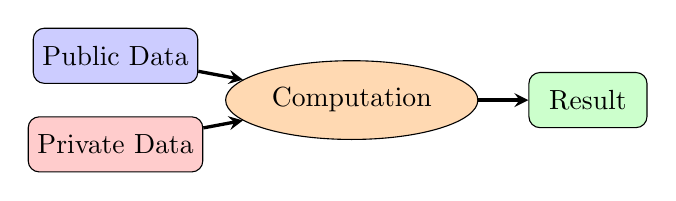
\begin{tikzpicture}[
    scale = 0.750,
      public/.style={draw, fill=blue!20, rectangle, rounded corners, minimum width=1.5cm, minimum height=0.7cm},
      private/.style={draw, fill=red!20, rectangle, rounded corners, minimum width=1.5cm, minimum height=0.7cm},
      computation/.style={draw, fill=orange!30, ellipse, rounded corners, minimum width=2cm, minimum height=1cm},
      result/.style={draw, fill=green!20, rectangle, rounded corners,  minimum width=1.5cm, minimum height=0.7cm},
      arrow/.style={->, >=stealth, very thick, color=black}
  ]
      % Public Data
      \node (public) at (0, 0) [public] {Public Data};

      % Private Data
      \node (private) at (0, -1.5) [private] {Private Data};

      % Computation
      \node (computation) at (4, -0.75) [computation] {Computation};

      % Result
      \node (result) at (8, -0.75) [result] {Result};

      % Arrows
      \draw[arrow] (public) -- (computation);
      \draw[arrow] (private) -- (computation);
      \draw[arrow] (computation) -- (result);
  \end{tikzpicture}
  \caption{An unverifiable process}


  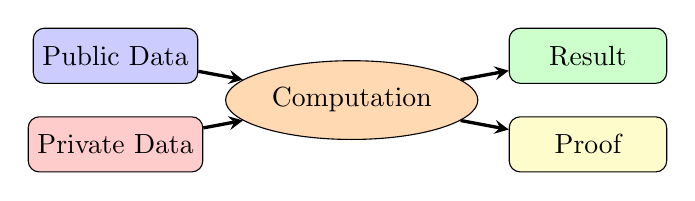
\begin{tikzpicture}[
    scale = 0.750,
    public/.style={draw, fill=blue!20, rectangle, rounded corners, minimum width=1.5cm, minimum height=0.7cm},
    private/.style={draw, fill=red!20, rectangle, rounded corners, minimum width=1.5cm, minimum height=0.7cm},
    computation/.style={draw, fill=orange!30, ellipse, rounded corners, minimum width=2cm, minimum height=1cm},
    result/.style={draw, fill=green!20, rectangle, rounded corners, minimum width=2cm, minimum height=0.7cm},
    proof/.style={draw, fill=yellow!20, rectangle, rounded corners, minimum width=2cm, minimum height=0.7cm},
    arrow/.style={->, >=stealth, very thick, color=black}
]
    % Public Data
    \node (public) at (0, 0) [public] {Public Data};

    % Private Data
    \node (private) at (0, -1.5) [private] {Private Data};

    % Computation
    \node (computation) at (4, -0.75) [computation] {Computation};

    % Result
    \node (result) at (8,  0) [result] {Result};

    % Proof
    \node (proof) at (8, -1.5) [proof] {Proof};

    % Arrows
    \draw[arrow] (public) -- (computation);
    \draw[arrow] (private) -- (computation);
    \draw[arrow] (computation) -- (result);
    \draw[arrow] (computation) -- (proof);
\end{tikzpicture}
\caption{A verifiable process}


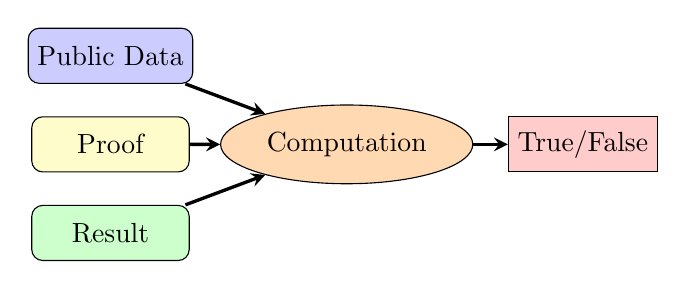
\begin{tikzpicture}[
  scale = 0.750,
  public/.style={draw, fill=blue!20, rectangle, rounded corners, minimum width=1.5cm, minimum height=0.7cm},
  proof/.style={draw, fill=yellow!20, rectangle, rounded corners, minimum width=2cm, minimum height=0.7cm},
  result/.style={draw, fill=green!20, rectangle, rounded corners, minimum width=2cm, minimum height=0.7cm},
    computation/.style={draw, fill=orange!30, ellipse, minimum width=2cm, minimum height=1cm},
    boolean/.style={draw, fill=red!20, rectangle, minimum width=1.5cm, minimum height=0.7cm},
    arrow/.style={->, >=stealth, very thick, color=black}
]
    % Public Data
    \node (public) at (0, 0) [public] {Public Data};

    % Proof
    \node (proof) at (0, -1.5) [proof] {Proof};

    % Result
    \node (result) at (0, -3) [result] {Result};

    % Computation
    \node (computation) at (4, -1.5) [computation] {Computation};

    % True/False
    \node (boolean) at (8, -1.5) [boolean] {True/False};

    % Arrows
    \draw[arrow] (public) -- (computation);
    \draw[arrow] (proof) -- (computation);
    \draw[arrow] (result) -- (computation);
    \draw[arrow] (computation) -- (boolean);
\end{tikzpicture}
\caption{Verification part of a verifiable process}

\end{wrapfigure}


As the reader can see that privacy and verifiability 
are conflicting requirements, and the only way to reconcile them 
is to use cryptographic techniques. Therefore, 
if every hospital, with their model, also provide 
a (cryptographic) proof of training on the legitimate data, then everyone 
can check the proof to ensure the correctness of the computations. 
In verifiable process scenario, each hospital can verify to others that 
they trained their model on legitimate data without sharing it by 
checking the proof; therefore, it is both private and verifiable. 
This, however, is just an example where we need both privacy and 
verifiability, and there are numerous other real-world examples, 
e.g., electronic-voting where we want to declare 
the right winner without disclosing the contents of cast ballots, 
auction server where you want to declare the winning 
bid releasing the highest bid but not disclosing the 
other bids, age-verification where you want to just verify 
that a user is over 18 without disclosing their date of birth, etc. 




On one hand, researchers have attempted to solve simpler version of 
these problems, e.g., 
enabling users to access online 
services without revealing their identity \cite{10.1145/586110.586114},
building privacy into electronic ID cards \cite{10.1145/2133375.2133379},
managing health information \cite{10.1145/3338854},
smart energy grids  \cite{LIN2021103505}, enabling e-voting systems \cite{doesburg2020using}, etc. 
None of these methods, however, are expressive enough to do arbitrary
computation that many businesses need. On the other, 
the recent development in the verifiable computing and zero-knowledge proof, 
in particular zero-knowledge succinct non-interactive argument of knowledge (zk-SNARK) 
\cite{10.1007/978-3-642-17373-8_19, 10.1007/978-3-642-38348-9_37, 
ben2013snarks, parno2016pinocchio, groth2016size, 10.1007/978-3-642-36594-2_18,
10.1007/978-3-662-44381-1_16, 8418611, 10.1007/978-3-030-17653-2_4, 10.1145/3319535.3339817,
cryptoeprint:2019/953, 10.1007/978-3-030-45721-1_26, 10.1007/978-3-030-56877-1_25}, 
has led to many useful privacy preserving applications, e.g., 
anonymous payment \cite{6956581}, privacy-preserving smart-contracts \cite{7546538},  
decentralised cryptocurrency \cite{cryptoeprint:2020/352}, etc., where 
arbitrary computation can be performed in privacy preserving, yet verifiable, manner. 
Unfortunately, most of these applications are focussed on cryptocurrencies. 

\textbf{Objective:} Therefore, the overarching goal of this
project is to explore and develop new zero-knowledge proof techniques for 
arbitrary computation on sensitive data for social good while preserving the privacy and ensuring the verifiability. 

\begin{enumerate}
  \item As a first phase, we aim to understand the personal data collection, storage, and their 
  purpose for which it is used by businesses and government bodies in Australia. 
  \textbf{Outcome:} new knowledge about the data collection practices in Australia. 
  (Phase 1, Year 1)
  \item In the second phase, we intend to understand if the existing zero-knowledge proof techniques 
  can be applied to achieve and scale the current business needs in Australia. If not, 
  then how to amend and optimise the existing techniques to cater the business needs of Australia.
  \textbf{Outcome:} new techniques for privacy preserving computation that suits business needs to Australian 
  companies and government entities (Phase 2, Year 2 and 3) 
  \item In the third, and final, phase, we intend to implement our methods 
  and prove them mathematically secure and trustworthy in the Coq theorem prover. 
  This step is crucial to bridge the gap between theoretical mathematical proofs and 
  practical implementation, increasing our confidence in the security and trustworthiness 
  of our approach. \textbf{Outcome:} mathematically proven correct computer program 
  as a proof of concept to demonstrate the feasibility of our approach
  (Phase 3, Year 2 and 3)
\end{enumerate}



\subsection*{Background on Zero-Knowledge Proof}
\textbf{In this section, when the reader encounters the word *proof*, think of it as data, in fact a large number}.
The notion of zero-knowledge proof is introduced by Shafi Goldwasser, Silvio Micali,
and Charles Rackoff in 1985 \cite{10.1145/22145.22178}. Informally, zero-knowledge proof 
provides an effective way of presenting the correctness of an assertion without revealing the actual proof.
They are extensively used in applications where privacy and 
verifiability, both, are needed, e.g., voting, authentication, cryptocurrencies, etc. 
First efficient construction of zero-knowledge proof is the Schnorr protocol \cite{schnorr1991efficient}, 
which we explain next for a brief context about zero-knowledge proofs. 

\begin{wrapfigure}{r}{0.40\textwidth} %this figure will be at the right
  \centering
\includegraphics[scale=0.4]{sigma.jpeg}
\caption{Sigma Protocol}
\label{fig:sig}
\end{wrapfigure}

In this protocol we have two parties, a prover $P$ and a verifier $V$. $P$ wants to convince 
$V$ that she knows the discrete logarithm $x$ of some group element $h$ such $h = g^x \in G$
where $G$ is a group of prime order $q$. In this setting, $g, h,$ and $G$ are public values, known 
by both $P$ and $V$ while $x$ is a secret value only known to $P$. (In this setting, computing 
discrete logarithm is a computationally difficult problem and no polynomial time 
Turing machine can compute the $x$, given $g$ and $h$).
The interaction 
is shown in the figure \ref{fig:sig}. In this interaction, $P$ picks a random number 
$r$ and computes $u = g^r$ and sends $u$ to $V$. In the second step, after receiving $u$, $V$ picks 
a random number $c$ and sends it to $P$.  Finally, $P$ computes $z = r + c * x$ and sends it 
to $V$. $V$ accepts it if $g^z = u * h^c$, otherwise rejects it. As the reader can 
see that the protocol 
forced $P$ to use secret value $x$ in the final step and the 
final equation only involves public values. We can construct 
more sophisticated sigma protocols by composing them together \cite{cramer1996modular}
for many practical applications, e.g., voting \cite{adida2008helios, cortier2019belenios}.
Sigma protocol, like any other proof system, has 
completeness and soundness. In addition, it has one more property 
zero-knowledge. Informally, completeness ensures 
that every true statement can be proven, soundness ensures that 
false statement cannot be proven, and zero-knowledge ensures that 
there is no leak of information other than the statement is true or not.
Zero-knowledge is what makes sigma protocol amenable to privacy preserving computation 
because it does not leak any information about the secret, e.g., $x$ 
in the Schnorr protocol. 


For a long time, sigma protocol was used mainly in voting to achieve privacy and 
verifiability, but it was very inefficient.  However, \cite{groth2010short, 10.1007/978-3-642-38348-9_37} 
introduced an efficient zero-knowledge succinct non-interactive argument of knowledge (zk-SNARK) 
to achieve privacy and verifiability by 
improving the underlying ideas of sigma protocol, and recently its usage has exploded 
in cryptocurrency domain. Its potential, however, is largely unexplored in application 
for social good and requires a thorough investigation. 


\subsection*{Background on the Coq Theorem Prover}
\textbf{In this section, when the reader encounters the word *proof*, think of it as an a piece of string, an abstract syntax tree}. 
The Coq theorem prover \cite{the_coq_development_team_2019_3476303} is a tool that facilitates two things: (i) ability to write 
mathematical definitions (computer program is treated 
as mathematics in Coq) and (ii) ability to prove that the definitions are correct. For a long time,
Coq and other theorem provers like Isabelle, Lean, HOL4, etc., were only used in academic setting. 
However, in recent years, researchers have started using theorem provers to 
prove real-world computer programs for correctness, e.g., fiat-crypto \cite{8835346}, 
a mathematically proven correct cryptography library in Coq, is 
used in Firefox and Chrome, HACL* \cite{10.1145/3133956.3134043}, another 
mathematically proven correct cryptography library in F*, used in  Mozilla's NSS cryptographic library, 
CompCert \cite{Blazy-Leroy-05}, a mathematically proven correct C compiler, is used by many 
companies\footnote{https://www.absint.com/success.htm}, 
Verified Software Toolchain \cite{10.1007/978-3-540-74591-4_3}, a mathematically proven correct tool in Coq, 
used to prove that a 25 years old 
in library is correct \cite{10.1007/978-3-031-13188-2_14}, and SeL4 \cite{10.1145/1743546.1743574}, a formally 
verified operating system in Isabelle/HOL, and many more. 
Our reason to use the Coq theorem prover is because our privacy-preserving 
methods will deal with sensitive personal data and therefore we would 
like to mathematically establish that it is secure and trustworthy. 
I am an expert in Coq and have used it prove many real-world computer programs. 


\begin{wrapfigure}{r}{0.30\textwidth} %this figure will be at the right
  \centering
\includegraphics[scale=0.4]{coq.jpeg}
\caption{List Encoding in Coq}
\label{fig:coq}
\end{wrapfigure}


We give a brief example, shown in figure \ref{fig:coq}, where we prove that list concatenation is associate. 
The first step is to encode the definition of list and concatenation function, 
and finally we prove that list concatenation is associative. 
List data structure is defined as an inductive datatype (\textit{Inductive}), 
indicating that it can be constructed in two ways: either with 
\textit{Nil}, representing an empty list, or with \textit{Cons}, 
which combines an element with an existing list to create a new list.
Then we define a function, using the keyword \textit{Fixpoint}, 
\textit{concat} that takes two lists and combines them into a single list. 
In the Coq theorem prover, like in other languages, we define data types and functions. 
However, unlike traditional languages, we do not write test cases; instead, 
we prove the correctness of functions, e.g., in this case, 
we mathematically prove that the \textit{concat} function 
is associate (see the theorem \textit{List\_concat\_associative}).




\subsection*{\TitleFont PROJECT QUALITY AND INNOVATION}
\rules{This sub-section requires investigators to address the Selection Criteria 
(Project Quality and Innovation – 40\%). This section will need to provide: 
Detail around both significance and innovation}

\subsection*{Significance}
\rules{An explanation of how the project will effectively address a significant problem}
According to a study by Surfshark \cite{surfshark}, Australia ranks 4th in the list of data breaches. 
One reason for these breaches is that many Australian entities, businesses 
and government bodies, store sensitive data in plaintext, which can be accessed by 
anyone with the right permissions, to verify users and perform certain business 
operations. Unfortunately, they often fail to take adequate measures to protect 
this data. Fortunately, recent advancements in cryptography, particularly zk-SNARK technology, 
and its application in cryptocurrencies, where sensitive data remains on the user's 
computer, for anonymous payment have opened up new possibilities for privacy-preserving computation;
however, anonymous payment is not a very difficult problem.
On the other hand, coming up with privacy-preserving techniques that does 
not require to leave the personal data from a users' computer for a business operation 
is an arduous problem This DECRA project aims to understand and explore the 
role of zk-SNARK in privacy-preserving computation for public good. 
If funded, the outcome of this project will advance our understanding 
of zk-SNARK technology, paving the way for more secure and trustworthy 
applications in field of social good.

\subsection*{Innovation}
\rules{Evidence that the framework is innovative and original}
There has been applications of zk-SNARK in cryptocurrencies, but they 
are dealing with very simple problems. In fact, their only problem is 
to ensure that a person doing a transaction has sufficient funds without revealing it (privacy 
and verifiability). However, compare this problem with a secure-voting problem where 
an election is conducted and ballots are encrypted, and an election commission 
has included only the correct ballots in the final tally and discarded 
all the incorrect ballots. The challenge here is for the election commission 
to convince voters that the final tally only includes the correct ballots and 
not the incorrect ones (privacy and verifiability). This turns out 
to be a very difficult problem, especially for voting system used in Australia such 
as Single Transferable Vote (STV). We are yet to see any application of 
zk-SNARK for public good, partly because a lot of problems that pertains to public are difficult. 
Therefore, it will take a significant amount of work and new knowledge creation to figure out a 
protocol required for privacy-preserving computation.


\rules{Detail around the conceptual framework, design and methods to demonstrate that they 
are adequately developed, well integrated innovative and original.}

\textbf{Project Methodology:} The research methods for this DECRA project 
relies on cryptography and mathematical logic (theorem proving). Our 
techniques for privacy preserving computing come from cryptography, 
while their proof of security and trustworthiness come from mathematical logic. 

\textbf{Phase 1 (Year 1):}
During this phase, our goal is to basically understand the Australian landscape of 
data collection and their purpose by businesses and government bodies.
In this phase, we aim to gain deep understanding of data collection in few areas, such 
as healthcare, finance, and social benefits. 
The requirements will be thoroughly investigated using the 
existing literature, as well as collaborative efforts with partners in the 
industry, government, and academia. This approach will ensure a comprehensive 
understanding of the necessary criteria and insights from diverse perspectives.


\textbf{Phase 2 (Year 2 and Year 3):}
During this phase, our goal is understand the existing methods such as 
\cite{groth2016size, Bowe2019HaloRP, Gabizon2019PLONKPO}. 

\textbf{Phase 3 (Year 2 and Year 3):}













\rules{How the research will maximise benefits to Australia, and if relevant, how it 
addresses any Science and Research Priorities (and associated Practical Challenges).}
This research, if funded, tackles one of the most difficult and pertinent problems  
of Australian Society, personal data leak. In addition, our findings can be used 
by Australian tech companies to develop privacy-preserving solutions. 
We emphasize that one of the reasons we want to prove our techniques mathematically 
is to ensure that in the future our protocols are not broken, 
thus safeguarding the investments made by Australian companies.
We want to prove once and forall that our method and its implementation 
is trustworthy and can be used without any repercussions. 

\rules{Describe the extent to which the proposal will advance knowledge.}
The proposal to explore the recent advancements in zk-SNARK (zero-knowledge succinct non-interactive argument of knowledge) 
technology for social good offers a substantial advantage for data privacy. 
Their potential have largely been unexplored 

zk-SNARKs are cryptographic techniques that enable the verification of the truth of 
a statement without revealing the underlying data. This advancement can significantly 
bolster privacy in various social contexts, such as healthcare, biometric, banking, etc. 
Allowing business users to prove possession of specific information without disclosing 
the information itself requires a significant amount of research 


\rules{Describe the potential for the research to enhance international collaboration.}
This project will collaborate with Bas Spitters at Aarhus University, Denmark, 
Véronique Cortier and Steve Kremer at CNRS, France, Adam Chilipala at MIT, USA, 
Vincent Cheval at the University of Oxford, UK, 
Clément Pit-Claudel and Bryan Ford at EPFL, and Thomas Haines and Dirk 
Pattinson at the Australian National University. 







\subsection*{BENEFIT}
 We have reached to a point where we can use the existing techniques for social good. 
 There are already many companies that working in the space of anonymous cryptocurrencies (cite them) 
 using the cutting-edge cryptographic techniques, it is imperative that we 
 try to analyse these technique and optimise the existing one, or invent new one, 
 that can be used to solve problem that matters to people. In the process, 
 I will create new knowledge (protocols) that can be commercialised and used 
 by Australia companies to lead to privacy front, given that the world 
 is moving towards privacy preserving computing. In addition, 
 they don't need to keep the data on their premises and therefore 
 reducing the risk on data-breach. 


\subsubsection{Social Benefit}
  A lot of online frauds happen because people's personal data is already present 
  online. However, if we can devise a system where we don't need to give data 
  but do the business as usual then it will make the data breach, or make them 
  obsolete, meaningless because there won't be a data to leak. This project 
  is a step towards empowering the society to control their 
  personal data. 

\subsubsection{Commercial Benefit}
  As the voice for privacy and ethical business is growing around the world, 
  it would be good idea for Australian business to take a lead. They should 
  focus on privacy-preserving computing because it provides almost 
  the same functionality as keeping the plaintext data at their premises. 
  This would reduce the cost of keeping data onhouse and ensuring 
  the security. 




\subsection*{COMMUNICATION OF RESULTS}
The results from this project will primarily be published in security and theorem proving conferences, 
such as ACM Computer and Community Security (CCS), USENIX Security, IEEE Security and Privacy (S\&P), 
Computer Security Foundations symposium (CSF), Privacy Enhancing Technologies Symposium (PETS),
IEEE European Symposium on Security and Privacy (EuroS\&P), Interactive Theorem Proving (ITP),
and Certified Programs and Proofs (CPP). In addition, the Coq source code developed during this project 
will be made public available on my homepage and my GitHub profile with permissive license. 




\subsection*{Investigator/Capability}
My research touches the lives of common people and solves
real-world problems that matter to democracies and common people. During my 7 years research career 
--ranging from Australian National University, University of Melbourne, University of Cambridge, 
and University of Oxford-- I have produced 9 mathematically proven correct 
software for public good, which includes software to count Australian Senate election ballots,
mix-network used in Switzerland election, software for both: plaintext ballot Schulze Method and 
encrypted ballot Schulze method, software to process sensitive data in trusted 
computing (Intel SGX and ARM Trustzone), software to model cryptographic protocols, 
software to verify the integrity of elections conducted by International Association for Cryptologic Research, 
software to model networking-protocols, software to bootstrap an election by 
producing independent group generators, and software to model Helios voting system.

In this section, I briefly explain my papers and how they solve a problem pertaining to social good.
My paper (i) \textbf{Assume but Verify: Deductive Verification of Leaked Information in Concurrent Applications} \cite{murrayassume},
accepted in ACM CCS 2023, develops a theory
for processing sensitive data --ethnic origin, political opinions,
health-related data, and  biometric data-- of common
people in secure enclave, e.g., Intel SGX, Arm TrustZone, etc. Moreover,
we demonstrate the usability of our method by developing non-trivial case studies that handles
sensitive data accompanied by the machine-checked mathematical proofs that none of
them have unintended side-channel data leakage;
(ii) \textbf{Machine-checking Multi-Round Proofs of Shuffle: Terelius-Wikstrom and Bayer-Groth} \cite{287095},
published in USENIX Security 2023, mathematically establishes a critical piece of
code in the SwissPost voting software --used in legally binding
elections in Switzerland-- is correct (and debunks a decade old myth of the cryptographic
community that Terelius-Wikstrom method is zero-knowledge proof. We have formally
proved in the Coq theorem prover that it is a zero-knowledge argument and not
a zero-knowledge proof);
(iii) \textbf{Verifiable Homomorphic Tallying for the Schulze Vote Counting Scheme} \cite{10.1007/978-3-030-41600-3_4}, published
in VSTTE 2019, not only developes a publicly verifiable method to count encrypted ballots for
a complex voting method but it
is also proven correct in the Coq theorem prover to ensure that there is no gap between
the pen-and-paper proof and the actual implementation;  (iv) \textbf{Verified Verifiers for
Verifying Elections} \cite{10.1145/3319535.3354247}, published in ACM CCS 2019, develops a mathematically proven correct tool
in the Coq theorem prover to verify the elections conducted by
the International Association for Cryptologic Research. We have used
our tool to verify the integrity of IACR elections; (v) \textbf{Modular Formalisation and
Verification of STV Algorithms} \cite{10.1007/978-3-030-00419-4_4}, published in E-Vote 2018, develops a mathematically proven
correct tool in the Coq theorem prover. We have used this tool to verify
the results of Australian Senate election;
(vi) \textbf{Verifpal: Cryptographic Protocol Analysis for the Real World} \cite{10.1007/978-3-030-65277-7_8}, published in
INDOCRYPT 2020, develops a tool that can used to model real work cryptographic protocol.
Verifpal has been used by many researchers to model security and privacy aspect of
digital contact tracing during COVID; (vii) \textbf{Schulze Voting as Evidence Carrying Computation} \cite{10.1007/978-3-319-66107-0_26}, 
published in ITP 2017, develops the idea of proof-carrying computation for 
the Schulze Method, one of the widely used method over the Internet. 
At the University of Cambridge, I developed a mathematically proven correct tool in 
the Coq theorem prover that can be used by researchers to model networking-protocols in the abstract
setting of semirings (and we are in the process of submitting our paper in CAV 2024).
At the University of Oxford, I am exploring the avenues to bridge the gap between a security protocol
(formal communication model) with its implementation using session types, and our
goal is to produce a more realistic distributed executable model of the security protocol.
Currently, as a first step, I am focussing on Signal app
where my goal is to prove (or disprove) that its Java implementation follows the
communication model described in the Signal's documentation.
In a nutshell, all my research so far has an impact on the lives on common people and
researchers and my DECRA proposal is a step towards continuing my research 
for the social good. 

\subsubsection*{National Interest Test Statement}
According to a study by Surfshark, Australia ranks 4th in the list of data breaches. 
One reason for these breaches is that many Australian entities, businesses 
and government bodies, store sensitive data in plaintext, which can be accessed by 
anyone with the right permissions, to verify users and perform certain business 
operations. Unfortunately, they often fail to take adequate measures to protect 
this data. Fortunately, recent advancements in cryptography enable us to verify 
users and conduct most business operations without storing data on-site. In fact, 
these techniques ensure that data never leaves the users' computers, eliminating the risk of data breaches. 
Through this project, we will investigate the collection of personal data by businesses 
and government bodies in Australia and their intended purposes. Additionally, we will 
explore recent advancements in cryptographic technology to perform business 
operations without the need to store personal data. 
This research will benefit the Australian community by developing privacy-preserving technology 
which will enhance personal data security. We also hope that our study will 
contribute to the development of Australia's policies regarding personal data collection.



%\vspace{4pt}
\renewcommand{\refname}{\normalfont\selectfont\TitleFont REFERENCES} 
%\vspace{-14pt}
\begingroup
    \fontsize{10pt}{10pt}\selectfont
\bibliographystyle{abbrv}
\bibliography{references.bib}



%\todo{\subsection*{Changes to be made}}
%\todo{
%\begin{enumerate}
%\item bring clear aims, objectives and methods in the first page
%\item clarify how the method is unique, why cannot be done by Google or others. Clarify why it leads to a solution
%\item reduce the quantity of text
%\item add images: 1. example of good query and results vs example of bad query and result; 2. study methodology/phases
%\end{enumerate}}


\endgroup


\end{document}


